\section{Introduction}
The FCC-ee high-luminosity circular electron-positron collider, with center-of-mass energies $\sqrt{s}$ from $91.2\,\gev$ to
$365\,\gev$, allows for high-precision measurements of the properties of the Z, the W, the top quark and the Higgs boson. As a predecessor of a new $100\,\tev$ proton-proton collider, the FCC-ee collider is foreseen to be placed in a 100~km tunnel in Geneva area as shown in~\cref{fig_fcc_cern}.

\begin{figure}[ht]
	\centering
	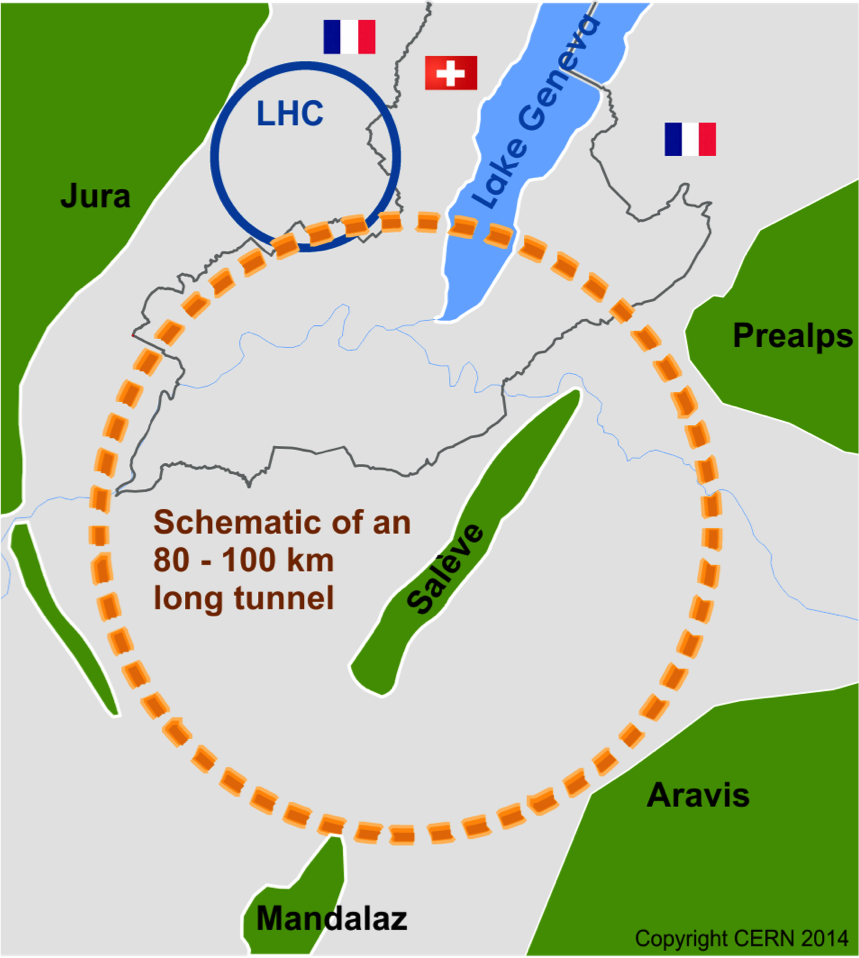
\includegraphics[width=0.3\textwidth]{figures/cernFCC.jpg}%
	\caption{A possible realization of the FCC experiment near the Geneva region.}
	\label{fig_fcc_cern}
\end{figure}

The IDEA detector, one of the two detector concepts under development for FCC-ee, has demanding requirements to match the experimental conditions. Its main components consist of: an ultra-light silicon-based vertex detector, an ultra-light drift chamber for track reconstruction and particle identification, a dual-readout calorimeter, a 2~T axial magnetic field and an instrumented return yoke as illustrated in~\cref{fig_IDEA}. The drift chamber is being investigated using \textsc{Geant4}-based simulations. Its performance and the effect of beam-induced backgrounds are presented here-below.

\begin{figure}[ht]
	\centering
	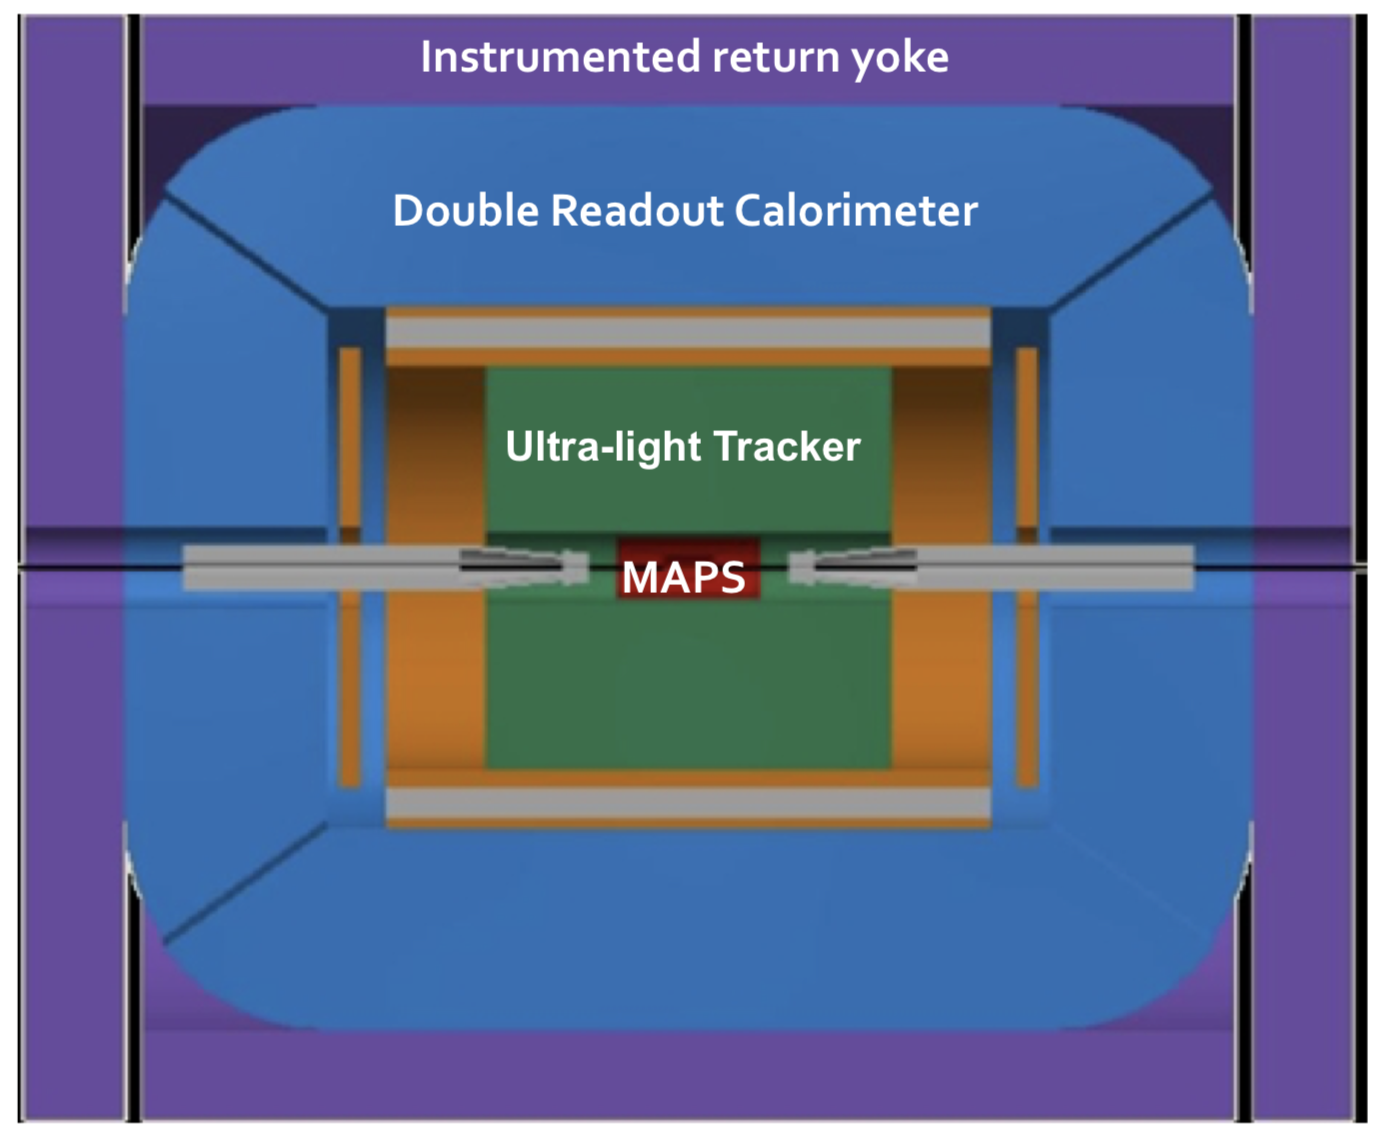
\includegraphics[width=0.5\textwidth]{figures/FCCeeIDEAConcept}%
	\caption{Schematic layout of the IDEA detector with the sub-detectors illustrated in different colors: vertex detector (red), drift chamber (green), pre-shower (orange), magnet (gray), calorimeter (blue), magnet yoke and muon system (violet).}
	\label{fig_IDEA}
\end{figure}

\section{Drift chamber}
The drift chamber (DCH) is optimized to provide excellent tracking, high precision momentum measurement and excellent particle identification using cluster counting technique with an extremely low material content.

The drift chamber for IDEA is based on the drift chamber for the KLOE experiment~\cite{DeLucia:2018qoc} as well as a more recent version of it developed for the MEG2 experiment~\cite{Baldini:2018nnn}.

The drift chamber consists of a unique-volume with high granularity. It is foreseen to use a gas composed of $90~\%$ of Helium and $10~\%$ of isobutane ($\text{C}_{4}\text{H}_{10}$). It is composed of 112 co-axial layer with wires having an average stereo angle of 0.1~radians allowing for a longitudinal resolution of 1~mm. The square cell size varies between 12.0~mm and 14.5~mm. The parameters of the drift chamber for the IDEA detector are summarized in \cref{driftChamberParams}. The description of the simulation chain for the drift chamber using the FCCSW is described here-below.

\begin{table}[!t]
	\renewcommand{\arraystretch}{1.3}
	\caption{Parameters of the drift chamber for the IDEA detector}
	\label{driftChamberParams}
	\centering
	% Some packages, such as MDW tools, offer better commands for making tables
	% than the plain LaTeX2e tabular which is used here.
	\begin{tabular}{l l}
		\toprule
			Length & 4~m \\
      Inner radius & 0.345~m \\
      Outer radius & 2~m\\
      Number of sensitive wires & 56'448 \\
      Transverse resolution & 0.1~mm \\
			Longitudinal resolution & 1~mm \\
			Material content in radial direction & 1.6\% \\
			Material content in the forward direction & 5.0~\% \\
		\bottomrule
	\end{tabular}
\end{table}


\section{Simulation with the FCC Software}

The FCC Software (FCCSW)~\cite{FCCSW} is a common software for all FCC experiments. It is based on the Gaudi software framework~\cite{Gaudi} for parallel data processing, \textsc{Geant4} simulation toolkit~\cite{Geant4} and the DD4hep detector description toolkit for high energy physics~\cite{DD4hep}. The FCCSW simulation pipeline is summarized in \cref{simu_chain} and described here-below.

\begin{figure}[!h]
\centering
	\smartdiagramset{back arrow disabled=true, module minimum width=2cm, text width=2cm, module minimum height=1cm, module x sep=3cm}
	\scalebox{0.75}{
	  	\smartdiagram[flow diagram:horizontal]
	  	{%
	    	{Geometry\\DDhep}, Segmentation, {Geant4 \\simulation}, Digitization%
	  	}
  	}
\caption{The FCCSW simulation chain.}
\label{simu_chain}
\end{figure}




\subsection{Geometry description with DD4hep}
First, the geometry of the detector is described using the DD4hep simulation framework. The current implementation of the detectors in the interaction region for the IDEA detector is shown in \cref{fig_sim}. The interaction region consists of a beam pipe, a shielding solenoid, a luminosity calorimeter, a vertex detector and a drift chamber. The geometry of the drift chamber is defined as layers of gas. In order to increase the simulation speed, the individual wires are not physically placed in the simulation software and the segmentation takes them into account.

\begin{figure}[ht]
\centering
	\begin{tikzpicture}
		\node[anchor=south west,inner sep=0] (image) at
		(0,0){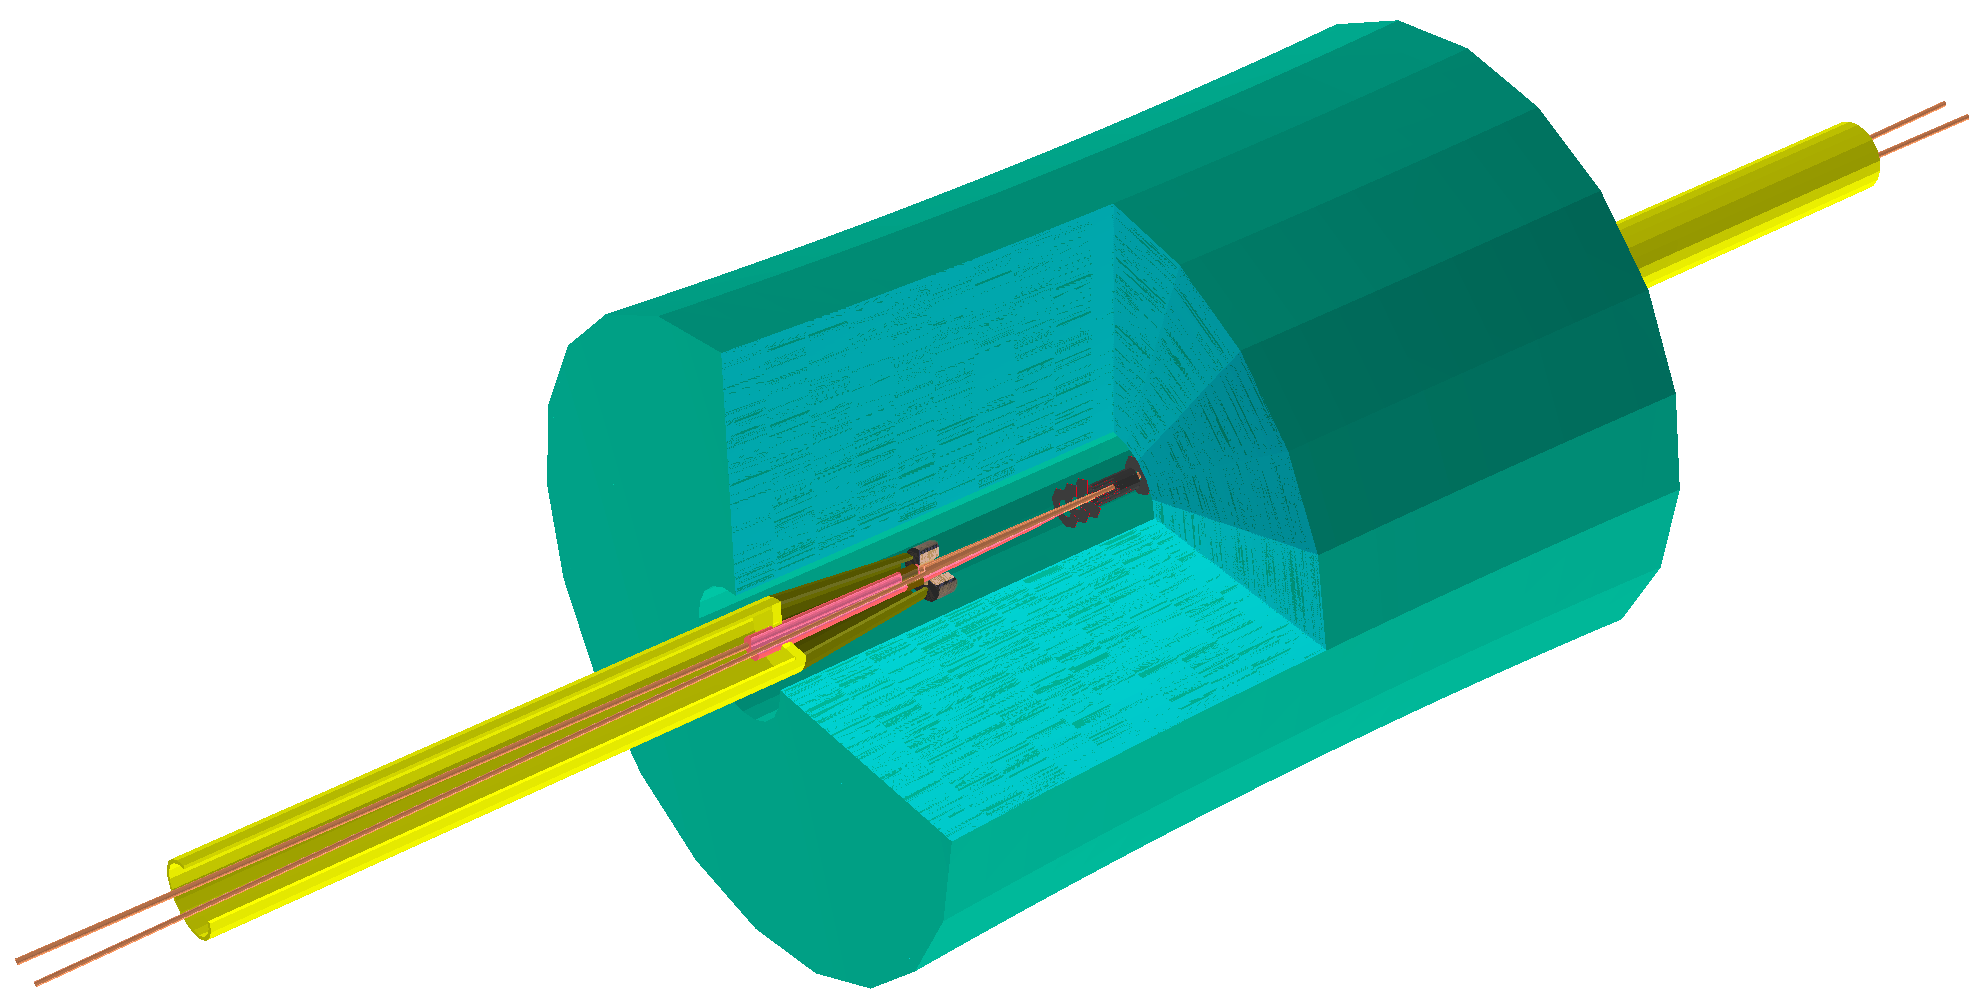
\includegraphics[width=0.8\textwidth]{figures/FCCeeIDEA_IR}};
		\begin{scope}[x={(image.south east)},y={(image.north west)}]
		\node[left] at (0.8, 0.7) {Drift Chamber};

		\draw[->, thick](0.05, 0.25) -- (0.05, 0.1);
		\node[above] at (0.05, 0.25) {Beam Pipe};

		\draw[->, thick](0.2, 0.45) -- (0.2, 0.22);
		\node[above] at (0.12, 0.45) {Solenoid Shielding};

		\draw[->, thick](0.3, 0.7) -- (0.42, 0.4);
		\node[above] at (0.2, 0.7) {Tungsten Shielding};

		\draw[->, thick](0.55, 0.05) -- (0.48, 0.4);
		\node[below] at (0.55, 0.05) {Luminosity Calorimeter};

		\draw[->, thick](0.75, 0.2) -- (0.58, 0.5);
		\node[below] at (0.75, 0.2) {Vertex Detector};

	\end{scope}
	\end{tikzpicture}

\caption{The detectors at the interaction region for the FCC-ee IDEA concept as implemented in FCCSW.}
\label{fig_sim}
\end{figure}

\subsection{Segmentation}

The segmentation of the sensitive gas detector contains the information on the positions of the wires in the detector. The segmentation for the first layer of the drift chamber is shown in \cref{fig_segmentation_first_case}. This reduces the running time by avoiding to place each wire volume individually.

\begin{figure}[ht]
	\centering
	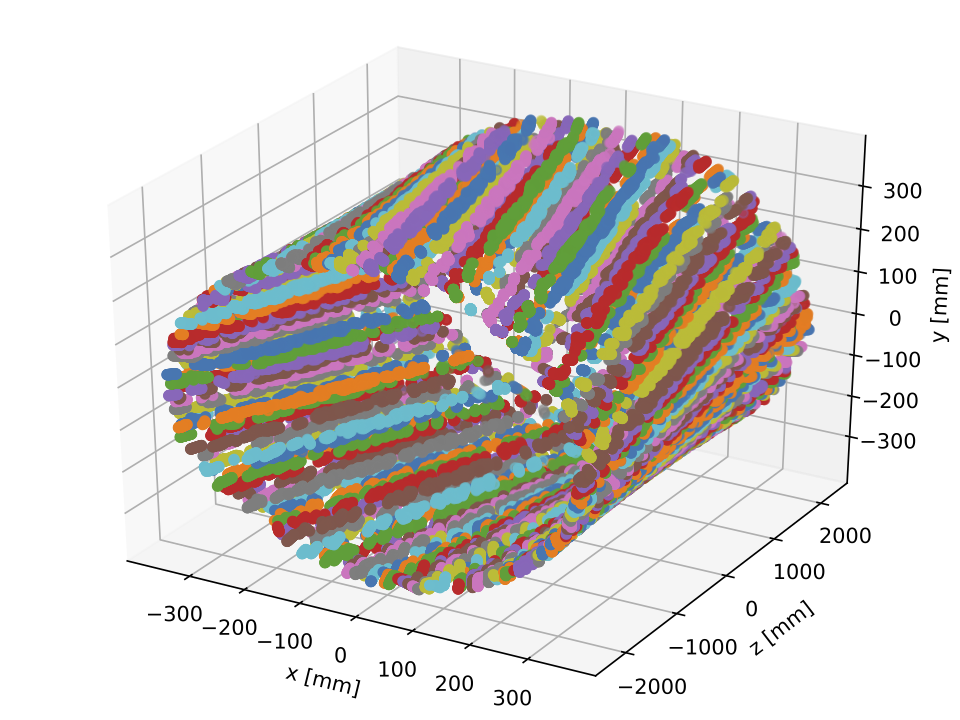
\includegraphics[width=0.6\textwidth]{figures/allHits}
	\caption{The segmentation of the first layer of the drift chamber.}
	\label{fig_segmentation_first_case}
\end{figure}

The total number of wires as a function of the polar angle $\theta$ is illustrated in \cref{fig_segmentation_second_case}. In the barrel region, a high coverage is obtained by $\sim~112$ wires in average. In the forward region, silicon disks are foreseen to improve the track angle coverage.

\begin{figure}[ht]
	\centering
	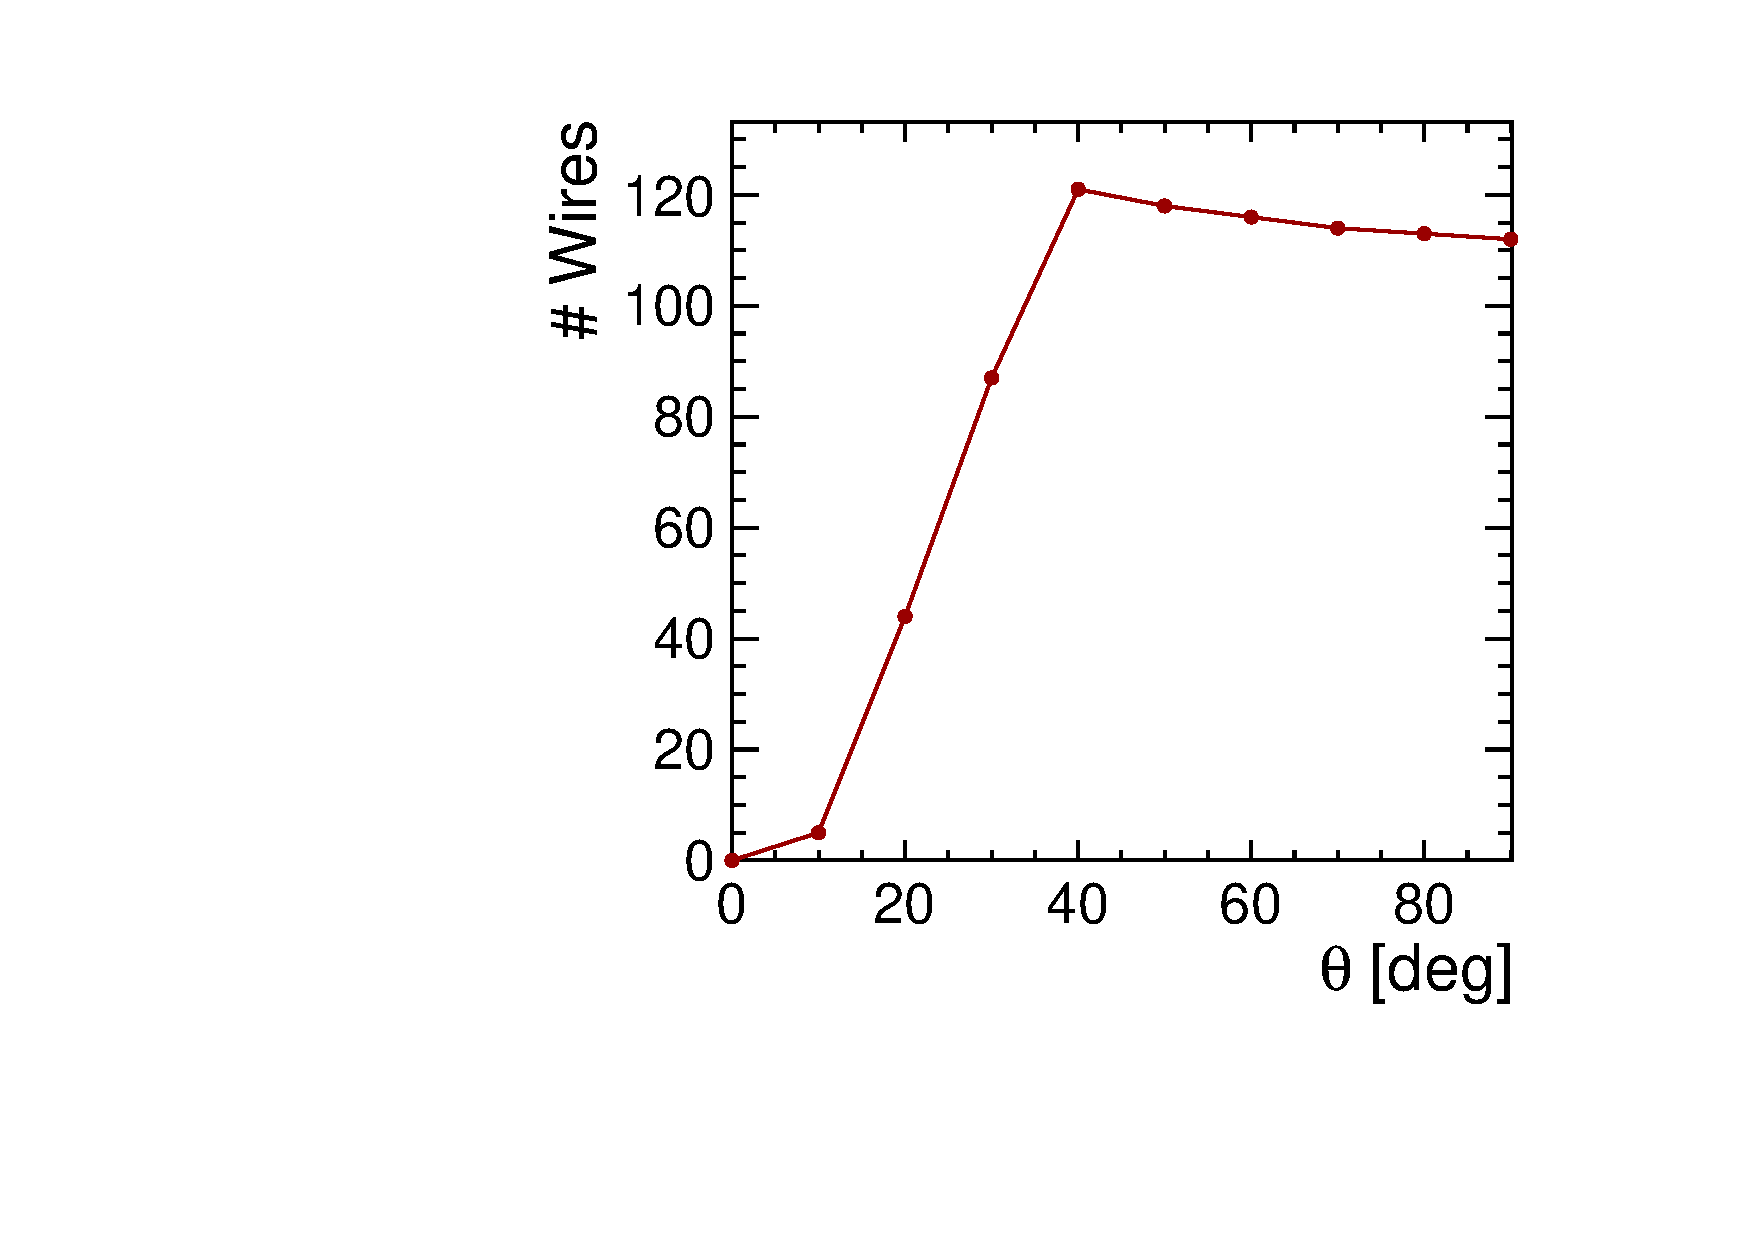
\includegraphics[width=0.6\textwidth]{figures/numWires}%
	\caption{Total number of wires as a function of the polar angle $\theta$ (calculated using infinite momentum tracks from the origin).}
	\label{fig_segmentation_second_case}
\end{figure}


\subsection{\textsc{Geant4} simulation and digitization}
\textsc{Geant4} simulates the passage of particles through matter. For the drift chamber simulation, a step size of 2~mm is chosen in order to step trough the gas volume and calculate the energy deposited. The ionization charge is then drifted to the nearest wire. This allows for calculating the drift time and therefore the signal in the wires. Once the contribution from each \textsc{Geant4} step is calculated, the digitization step regroups the energy deposited with a drift time smaller than the maximum drift time in the cell.

\section{Impact of beam-induced backgrounds}
Three main sources of beam-induced backgrounds at the FCC-ee experiment are: incoherent $e^+e^-$ pairs, $\gamma\gamma\rightarrow$~hadrons and the synchrotron radiation. Each background source is studied below.

The incoherent $e^+e^-$ pairs are generated from the strong electromagnetic force from the electron and positron bunches in the field of the opposite beam. This leads to the production of Beamstrahlung photons. The interactions of Beamstrahlung photons generate incoherent lepton pairs at low polar angles and mostly contained in the forward direction as shown in~\cref{fig_pairbcg}. The \textsc{GUINEA-PIG}~\cite{Schulte:382453} event generator has been used to generate the incoherent $e^+e^-$ background particles at a $\sqrt{s}$ of $91.2\,\gev$ and $365\,\gev$~\cite{Voutsinas:2017eca} and their impact on the drift chamber is simulated using the FCCSW. The occupancy of the drift chamber due to incoherent $e^+e^-$ pairs as a function of the detector radius is shown in~\cref{fig_simhitspercent}. In fact, the produced incoherent pairs have a low polar angle and only few of them reach the drift chamber. Most of the hits observed are due to the scattering of the $e^+e^-$ pairs by interacting with the elements in the interaction region.


\begin{figure}[ht]
\centering
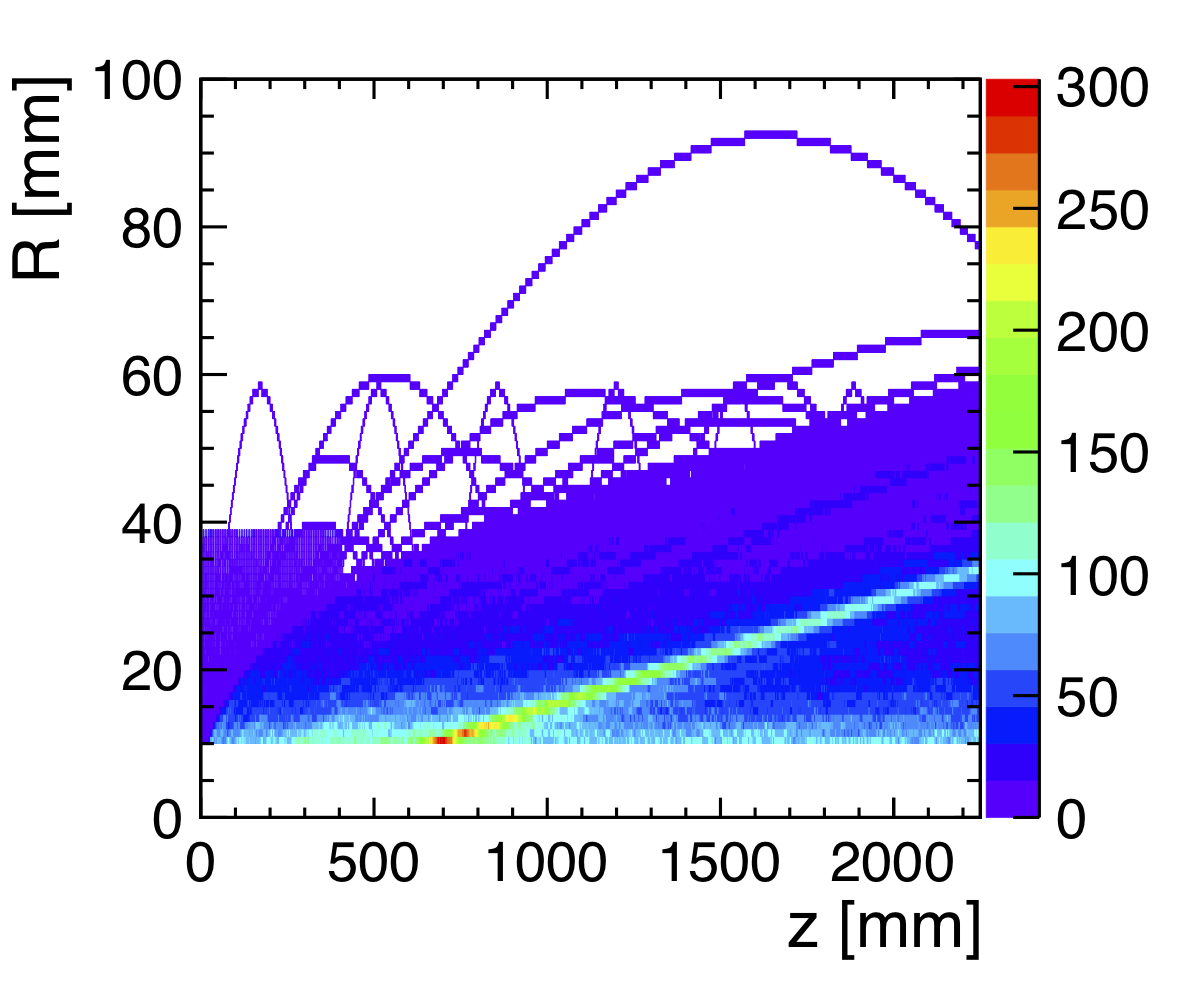
\includegraphics[width=0.6\textwidth]{figures/pairs_R_Z.png}
\caption{The trajectory of the $e^+e^-$ pairs in a 2~T magnetic field.}
\label{fig_pairbcg}
\end{figure}



The $\gamma\gamma\rightarrow$~hadrons background is expected to have a very low impact on the drift chamber. The synchrotron radiation, dictates the design of the interaction region. It defines the beampipe radius and the design of the shielding (in Tungsten).
\cref{occupancy_DCH} summarizes the occupancy in the drift chamber due to different sources of beam-induced backgrounds. The overall occupancy due to all backgrounds is as expected, with $e^+e^-$ pair background having the highest impact. Based on previous experience with the MEG2 experiment, it can be deduced that the background does not pose problem for the reconstruction of the tracks using the drift chamber.

\begin{figure}[ht]
\centering
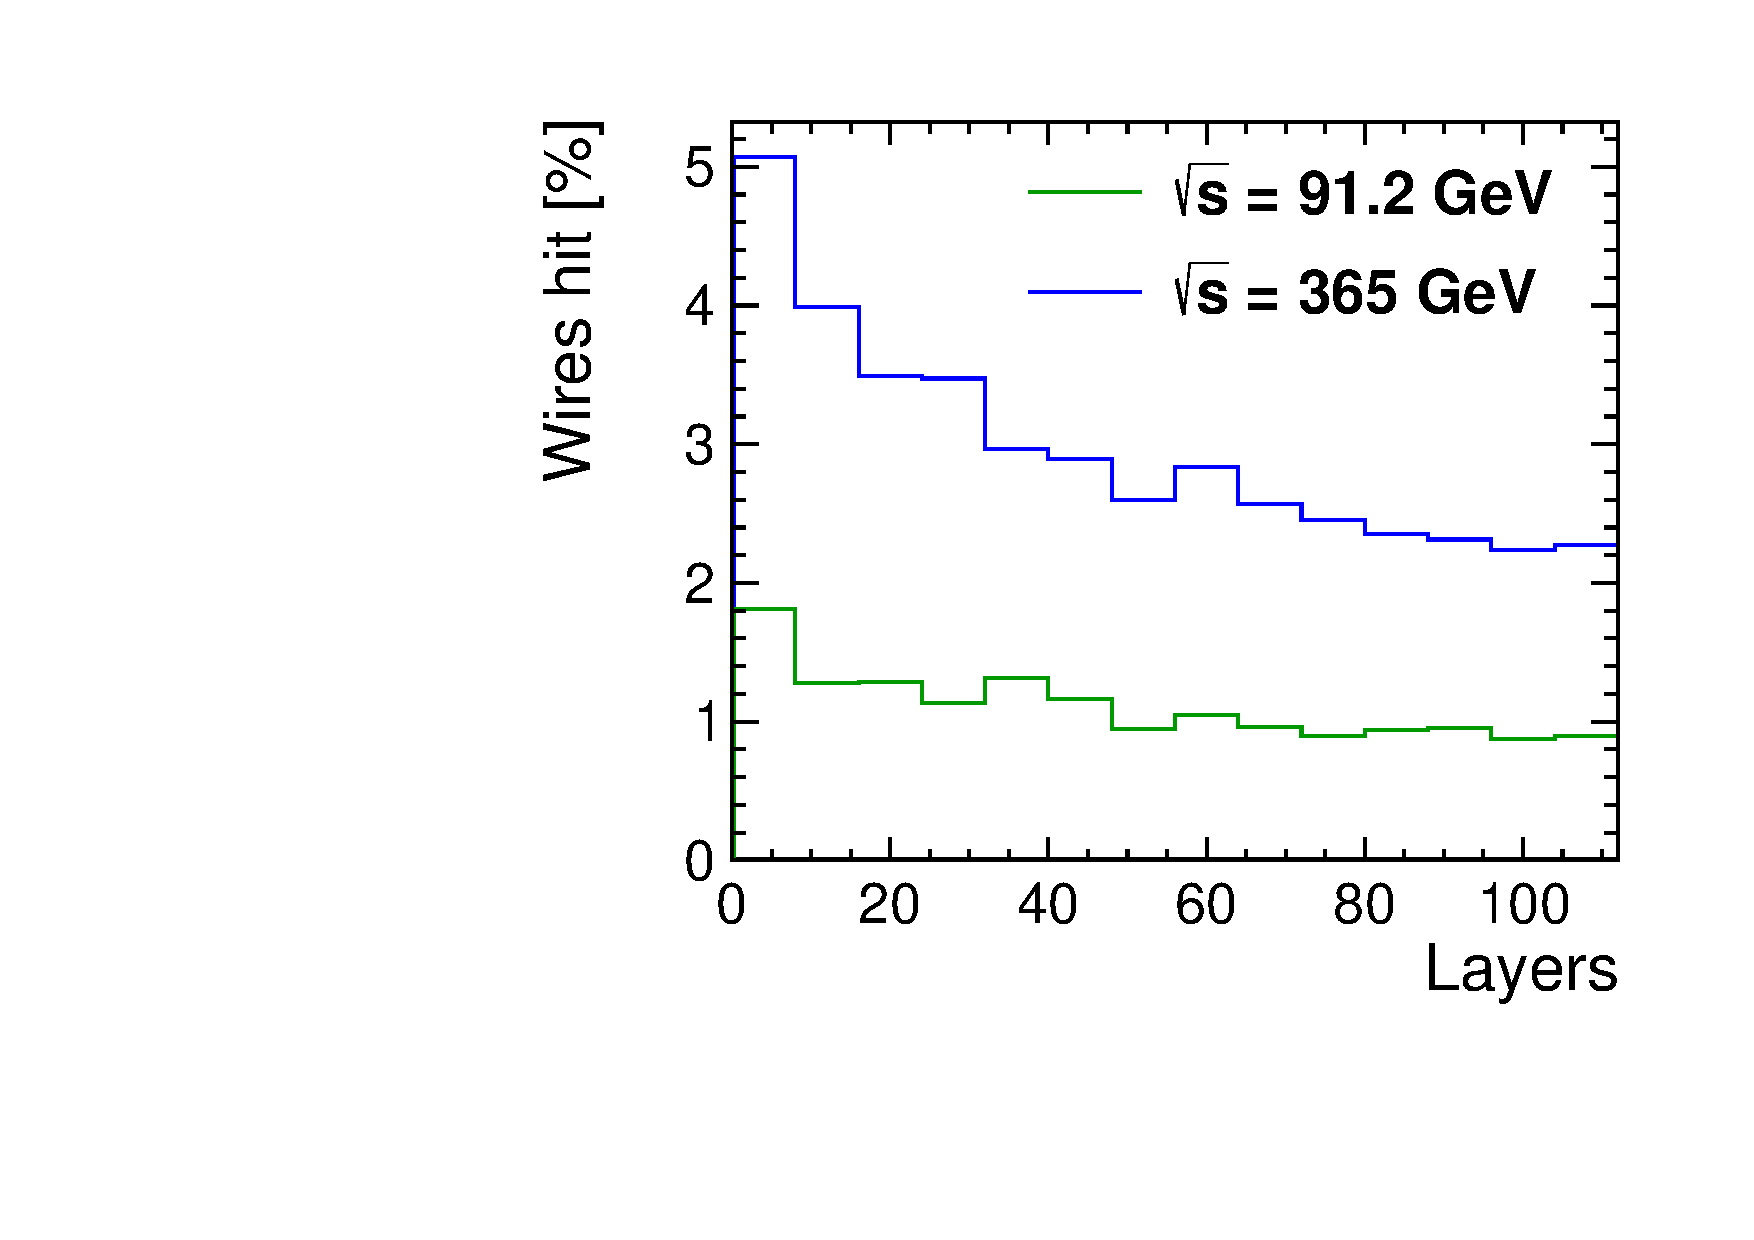
\includegraphics[width=0.6\textwidth]{figures/incoherent_top_Z.pdf}
\caption{The percentage of wires hit due to $e^+e^-$ pair background as a function of the layer radius averaged over 100 bunch crossings. For the Z stage ($\sqrt{s} = 91.2\,\gev$), the readout latency is also taken into account by summing up the background over 4 bunch crossings.}
\label{fig_simhitspercent}
\end{figure}

\begin{table}[ht]
	\renewcommand{\arraystretch}{1.3}
	\caption{Average occupancy in the drift chamber due to beam-induced backgrounds.}
	\label{occupancy_DCH}
	\centering
	\begin{tabular}{l c c}
		\toprule
		 Background & \multicolumn{2}{c}{Average occupancy} \\
			& $\sqrt{s}$ = 91.2~GeV & $\sqrt{s}$ = 365~GeV \\
		 \midrule
		 $e^+e^-$ pair background & 1.1\% & 2.9\% \\
		 $\gamma\gamma\rightarrow$ hadrons & 0.001\% & 0.035\%  \\
		 Synchrotron radiation & negligible & 0.2\% \\
		 \bottomrule
	\end{tabular}
\end{table}
